\chapter{The Burridge--Knopoff model}
\label{ch:bk}

This chapter presents the Burridge--Knopoff (BK) model in the form studied by Carlson,
Langer and collaborators~\cite{CarlsonLanger1989,Carlson1991}, and reviews their analysis.
We start from Newton's equations in physical units (\cref{sec:bk-eom}), reduce them to a
dimensionless form with only a few parameters (\cref{sec:bk-units}), and describe the two
friction laws used in the 1989 and 1991 papers (\cref{sec:bk-friction}). We then work out the
simplest motions of the model exactly (\cref{sec:bk-simple}), show why uniform sliding is
unstable (\cref{sec:bk-instability}), and follow Carlson and Langer's argument that leads to a
\emph{localization length}, the length that separates small, ``localized'' events from large,
``delocalized'' ones (\cref{sec:bk-pulses,sec:bk-localization}). The last part of the chapter
summarises the statistical results of the two papers, explains why they differ
(\cref{sec:bk-stats,sec:bk-differences}), and lists what a sandpile model would have to capture to
describe the BK model (\cref{sec:bk-summary}).

% ======================================================================
\section{Equations of motion}
\label{sec:bk-eom}

Consider the chain of \cref{fig:bk-sketch}: $N$ identical blocks of mass $m$, labelled
$j=1,\dots,N$, resting on a fixed rough surface. Let $X_j(t)$ be the displacement of block $j$ from
its position at time $t=0$, when all springs are relaxed. The upper plate moves with constant velocity
$v$, so at time $t$ it has moved by $vt$. Three kinds of forces act on block $j$:
\begin{itemize}
  \item \textbf{Coupling springs.} The spring to the right neighbour is stretched by $X_{j+1}-X_j$ and
    pulls block $j$ to the right with force $k_c(X_{j+1}-X_j)$; the spring to the left neighbour pulls
    with $k_c(X_{j-1}-X_j)$. Together:
    \begin{equation}
      k_c\,(X_{j+1} - 2X_j + X_{j-1}).
    \end{equation}
  \item \textbf{Pulling spring.} The leaf spring connecting the block to the plate is stretched by
    $vt - X_j$, the distance by which the plate has moved ahead of the block. It pulls the block
    forward with force $k_p\,(vt - X_j)$.
  \item \textbf{Friction.} The rough surface exerts a force $-F$ opposing the motion, described in
    \cref{sec:bk-friction}.
\end{itemize}
Newton's second law gives
\begin{equation}
  m\,\ddot X_j = k_c\,(X_{j+1} - 2X_j + X_{j-1}) + k_p\,(vt - X_j) - F_j ,
  \label{eq:bk-phys}
\end{equation}
where dots denote time derivatives. The first two terms together are the total \emph{spring force}
on the block, which we call $f_j$.

\paragraph{Boundary conditions.} Carlson and Langer use \emph{free} ends: the first and the last block
have only one coupling spring. This is expressed by defining $X_0\equiv X_1$ and $X_{N+1}\equiv X_N$ in
\cref{eq:bk-phys}, so that the missing spring exerts no force. (Setting $X_0 = X_{N+1}=0$ instead would
attach the end blocks to fixed walls, which is a different model.)

\paragraph{Friction.} The friction force depends on whether the block is moving:
\begin{itemize}
  \item A block at rest ($\dot X_j = 0$) is held by \emph{static} friction. Static friction takes whatever
    value is needed to keep the block at rest, $F_j = f_j$, as long as this is possible, i.e.\ as long as
    $f_j$ does not exceed the maximum static friction $F_0$. When $f_j$ reaches $F_0$, the block starts to
    slip.
  \item A slipping block feels \emph{kinetic} friction, which depends on its velocity:
    \begin{equation}
      F_j = F_0\,\phi\!\left(\frac{\dot X_j}{v_1}\right),
    \end{equation}
    where $\phi$ is a dimensionless function and $v_1$ is a characteristic velocity over which friction
    weakens. Since the surface is fixed, $\dot X_j$ is the velocity of the block relative to the surface.
\end{itemize}
A slipping block comes back to rest when its velocity returns to zero and the spring force is again within
the range that static friction can balance.

% ======================================================================
\section{Dimensionless form and the parameters of the model}
\label{sec:bk-units}

\Cref{eq:bk-phys} contains seven parameters: $m$, $k_c$, $k_p$, $F_0$, $v$, $v_1$ and the number of blocks
$N$. Many combinations of them give the same dynamics. To find the combinations that matter, we measure
time and displacement in natural units of the problem.

\paragraph{Unit of time.} A single block attached only to its pulling spring oscillates with angular
frequency $\omega_p = \sqrt{k_p/m}$. We use the dimensionless time
\begin{equation}
  \tau = \omega_p\, t .
\end{equation}

\paragraph{Unit of displacement.} A pulling spring exerts the maximum static friction force $F_0$ when it is
stretched by
\begin{equation}
  D_0 = \frac{F_0}{k_p} .
\end{equation}
This is the natural scale of slip: a block that slips releases a stretch of order $D_0$. We use the
dimensionless displacement $U_j = X_j/D_0$.

\paragraph{The dimensionless equation.} Substituting $X_j = D_0 U_j$ and $t=\tau/\omega_p$, time derivatives
become $\dot X_j = D_0\omega_p\,\dd U_j/\dd\tau$ and $\ddot X_j = D_0\omega_p^2\,\dd^2U_j/\dd\tau^2$. Inserting
this into \cref{eq:bk-phys} and dividing by $k_pD_0 = F_0$ (using $m\omega_p^2 = k_p$):
\begin{equation}
  \frac{m D_0\omega_p^2}{k_pD_0}\,\ddot U_j = \frac{k_c}{k_p}(U_{j+1}-2U_j+U_{j-1}) + \left(\frac{v}{D_0\omega_p}\,\tau - U_j\right)
  - \phi\!\left(\frac{D_0\omega_p}{v_1}\,\dot U_j\right),
\end{equation}
where dots now denote derivatives with respect to $\tau$. The coefficient on the left is 1, and we obtain
\begin{equation}
  \boxed{\;\ddot U_j = \ell^2\,(U_{j+1}-2U_j+U_{j-1}) + (\nu\tau - U_j) - \phi(2\alpha\,\dot U_j)\;}
  \label{eq:bk}
\end{equation}
with three dimensionless parameters:
\begin{equation}
  \ell^2 = \frac{k_c}{k_p},\qquad
  \nu = \frac{v}{\omega_pD_0},\qquad
  2\alpha = \frac{\omega_pD_0}{v_1}.
  \label{eq:bk-params}
\end{equation}
In addition there is the number of blocks $N$, and, for the 1991 friction law, the friction drop $\sigma$
introduced below.

\paragraph{Meaning of the parameters.}
\begin{itemize}
  \item $\ell^2 = k_c/k_p$ is the \emph{stiffness ratio}: how much stiffer the rock is along the fault than its
    connection to the driving plate. It sets how far the influence of one block reaches along the chain (see
    the continuum limit below). Simulations use $\ell$ between 3 and 12; for real faults Carlson and Langer
    estimate $\ell\sim100$.
  \item $\nu$ is the \emph{loading speed}: the plate velocity in units of the natural slipping velocity
    $\omega_pD_0$. Equivalently it is the ratio of the time a slip lasts ($\sim1/\omega_p$) to the time it takes the
    plate to load a pulling spring up to the threshold ($D_0/v$). For real faults $\nu\sim10^{-8}$ or less, as
    estimated in \cref{sec:stickslip}; simulations use $\nu = 10^{-2}$ to $10^{-3}$, or the limit $\nu\to0$.
  \item $\alpha$ measures \emph{how strongly friction weakens} with velocity: $2\alpha$ is the typical slipping
    velocity $\omega_pD_0$ divided by the velocity $v_1$ over which friction drops appreciably. Large $\alpha$
    means that a slipping block quickly loses most of its friction. Carlson and Langer argue that $\alpha$ is of
    order one, and use $1\le\alpha\le5$.
\end{itemize}

\paragraph{The frame of Carlson and Langer.} Carlson and Langer write the equations for the displacement
\emph{relative to the plate}, $U^{\text{CL}}_j = U_j - \nu\tau$. Since $\nu\tau$ is the same for all blocks it drops
out of the coupling term, $\dot U^{\text{CL}}_j = \dot U_j - \nu$, and \cref{eq:bk} becomes
\begin{equation}
  \ddot U^{\text{CL}}_j = \ell^2\,(U^{\text{CL}}_{j+1}-2U^{\text{CL}}_j+U^{\text{CL}}_{j-1}) - U^{\text{CL}}_j
  - \phi\bigl(2\alpha\nu + 2\alpha\dot U^{\text{CL}}_j\bigr),
  \label{eq:bk-CL}
\end{equation}
which is their Eq.~(2.5) (1989) and Eq.~(2.2) (1991). In this frame a stuck block moves backwards with the
surface, $\dot U^{\text{CL}}_j = -\nu$. The two forms are completely equivalent; we use \cref{eq:bk}, in which
stuck blocks are at rest.

\paragraph{Converting other units.} Simulations are often written with other choices of units, and the
parameters must then be converted with \cref{eq:bk-params} before results can be compared with the papers. For
example, a program that sets $m = F_0 = k_c = 1$, with pulling springs $k_p$ and kinetic friction
$F_0(1-\sigma)/[1 + c\,\dot X/(1-\sigma)]$, has $\omega_p = \sqrt{k_p}$ and $D_0 = 1/k_p$, so that
\begin{equation}
  \ell = \frac{1}{\sqrt{k_p}},\qquad \nu = v\sqrt{k_p},\qquad \alpha = \frac{c}{2\sqrt{k_p}},\qquad \tau = \sqrt{k_p}\,t .
\end{equation}
With $k_p = 0.04$ this gives $\ell = 5$ and $\alpha = 2.5\,c$: a friction coefficient $c = 1$ in such a program
corresponds to $\alpha = 2.5$, not to $\alpha=1$. The earlier version of this project used units of exactly this
kind, and this conversion is one of the reasons its results could not be compared directly with the papers.

\paragraph{The continuum limit and the stiffness length.} Let $a$ be the distance between neighbouring blocks,
and $s = ja$ the position along the fault. For displacements that vary slowly from block to block,
$U_{j+1}-2U_j+U_{j-1}\approx a^2\,\partial^2U/\partial s^2$, and \cref{eq:bk} becomes
\begin{equation}
  \ddot U = \xi^2\,\frac{\partial^2U}{\partial s^2} + (\nu\tau - U) - \phi(2\alpha\dot U),\qquad \xi = \ell a .
  \label{eq:bk-cont}
\end{equation}
Without friction and pulling springs this is a wave equation with wave speed $\xi$ (in units of length per unit
$\tau$): a disturbance travels $\ell$ blocks per unit time. The term $-U$ makes it a \emph{Klein--Gordon} (massive
wave) equation. The length $\xi$ also has a static meaning. If one block is pushed and the others are held by
static friction, the extra displacement $u$ of the chain obeys $\xi^2u'' - u = 0$ away from the push, so it decays
as $e^{-|s|/\xi}$: the influence of a perturbation extends over a distance $\xi$, about $\ell$ blocks. Beyond that
distance, the force has been absorbed by the pulling springs. This is the \emph{stiffness length}. Note that in
this chapter $\xi$ denotes the stiffness length, following Carlson and Langer; the length that plays the role of a
correlation length will be called $\tilde\xi$ (\cref{sec:bk-localization}).

\Cref{tab:bk-params} summarises the parameters.

\begin{table}[t]
\centering
\caption{Parameters of the BK model in the dimensionless form \cref{eq:bk}.}
\label{tab:bk-params}
\begin{tabular}{@{}lp{58mm}p{50mm}@{}}
\toprule
symbol & meaning & typical values \\
\midrule
$\ell^2=k_c/k_p$ & stiffness ratio; $\xi=\ell a$ is the stiffness length & simulations 3--12; real faults $\sim100$ \\
$\nu=v/(\omega_pD_0)$ & loading speed / slipping speed & real $\lesssim10^{-8}$; 1989: $10^{-2}$, $10^{-3}$; 1991: $\nu\to0$ \\
$\alpha=\omega_pD_0/(2v_1)$ & rate of velocity weakening & 1--5 \\
$\sigma$ & drop of friction at the onset of slip (1991) & $0.01$ \\
$N$ & number of blocks & 1989: 100--400; 1991: 4096--8192 \\
\bottomrule
\end{tabular}
\end{table}

% ======================================================================
\section{The friction laws}
\label{sec:bk-friction}

Both papers use the dimensionless friction $\phi(y)$, where $y=2\alpha\dot U$ is the sliding velocity in units of $v_1$
(\cref{fig:friction}).

\paragraph{The 1989 law.} In the first paper~\cite{CarlsonLanger1989} friction is symmetric:
\begin{equation}
  \phi(y) = \frac{\operatorname{sgn}(y)}{1+|y|}\quad(y\neq0),\qquad \phi(0)\in[-1,1].
  \label{eq:phi89}
\end{equation}
At rest, friction can take any value between $-1$ and $1$ (in units of $F_0$). When a block starts to slip forward,
friction is at first equal to its static maximum, 1, and then decreases: it falls to half at $y=1$, i.e.\ at the velocity
$v_1$, and to zero at large velocity. The slope at the start of slipping is $\phi'(0^+) = -1$. Blocks can also slip
backwards.

\paragraph{The 1991 law.} The second paper~\cite{Carlson1991} makes two changes:
\begin{equation}
  \phi(y) = \frac{1-\sigma}{1+y/(1-\sigma)}\quad(y>0),\qquad \phi(0)\in(-\infty,1].
  \label{eq:phi91}
\end{equation}
\begin{enumerate}
  \item At rest, friction can hold any backward force, so blocks never move backwards. The authors consider this more
    realistic.
  \item When a block starts to slip, friction drops \emph{immediately} from its static maximum 1 to $1-\sigma$. The initial
    slope is still $\phi'(0^+)=-1$.
\end{enumerate}
The second change is the important one. With the 1989 law, a block that reaches the threshold starts to move only
gradually, pushed by the slowly increasing spring force; how it starts depends on the loading speed $\nu$. With the
drop $\sigma$, a block at threshold experiences a net force $\sigma$ immediately and starts to slip abruptly, independently
of $\nu$. Slipping events then no longer depend on $\nu$ at all, and the limit $\nu\to0$ can be taken: the plate is
stopped while an event is in progress, and between events it is simply moved forward until the next block reaches
the threshold. This makes the simulation much more efficient, and it removes $\nu$ from the problem. As we will see,
$\sigma$ then takes over the role that $\nu$ played in the 1989 paper.

\begin{figure}[t]
  \centering
  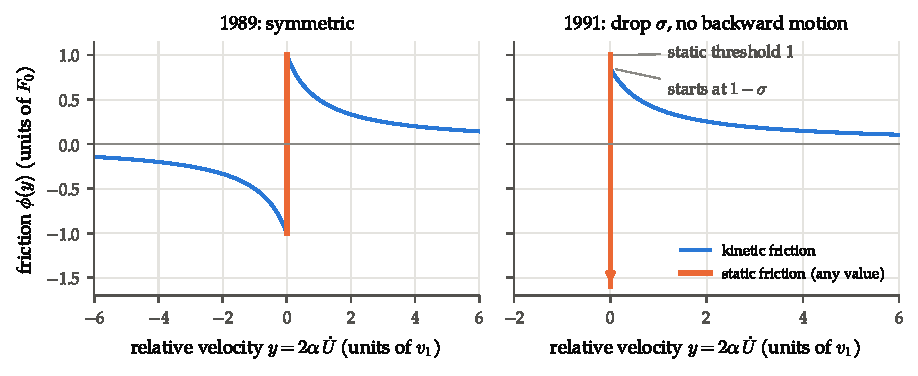
\includegraphics[width=\linewidth]{bk/friction.pdf}
  \caption{The friction laws of Carlson and Langer (1989, left) and of Carlson, Langer, Shaw and Tang (1991, right,
  drawn with $\sigma=0.15$ for visibility; the papers use $\sigma=0.01$). The vertical orange segments show the range of
  values that static friction can take at zero velocity.}
  \label{fig:friction}
\end{figure}

% ======================================================================
\section{Simple motions}
\label{sec:bk-simple}

\subsection{A single block: periodic stick--slip}

Consider first one block with no neighbours (or, equivalently, the whole chain moving rigidly). Its equation is
$\ddot U = (\nu\tau - U) - \phi(2\alpha\dot U)$. While it is stuck, the spring force $\nu\tau - U$ grows linearly with time.
When it reaches 1, the block slips.

If $\alpha$ is large, friction becomes small almost immediately, and the motion is approximately that of a free harmonic
oscillator, $\ddot U \approx \nu\tau - U$. Starting from the slip point, where $\nu\tau - U = 1$, and neglecting the plate
motion during the short slip, the solution is $U(\tau) = U_{\text{slip}} + 1 - \cos(\tau-\tau_{\text{slip}})$. The block
moves forward by 2 (in units of $D_0$) in a time $\pi$ and stops when its velocity vanishes; the spring force is then $-1$,
within the range of static friction, so the block sticks. The plate needs a time $2/\nu$ to load the spring again from
$-1$ to $+1$, and the cycle repeats. For smaller $\alpha$ friction removes part of the energy, and the slip is shorter.
\Cref{fig:single-block} shows the cycle computed numerically with the 1991 law for $\alpha=2.5$ and $\alpha=0.5$.

\begin{figure}[t]
  \centering
  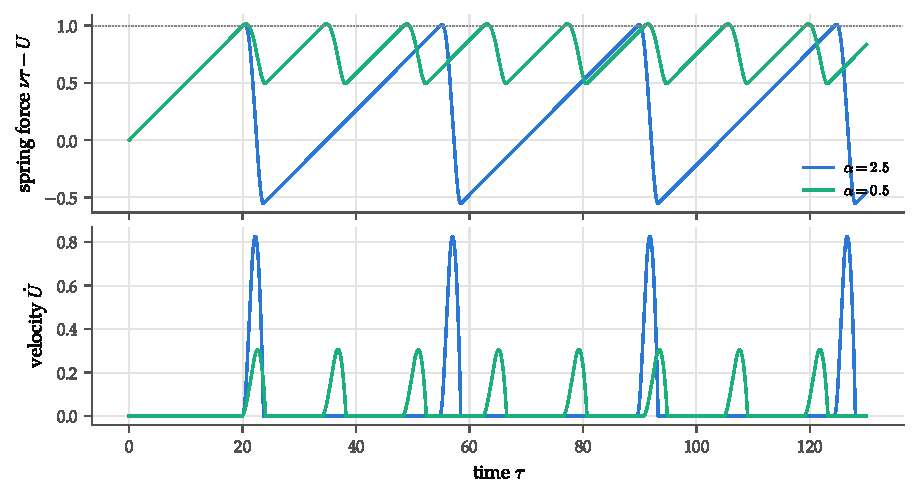
\includegraphics[width=\linewidth]{bk/single_block.pdf}
  \caption{Periodic stick--slip of a single block ($\nu=0.05$, $\sigma=0.05$). Top: spring force; the block slips each time it
  reaches the threshold 1 (dotted). Bottom: velocity. With strong velocity weakening ($\alpha=2.5$) each slip releases most of
  the stored force; with weak weakening ($\alpha=0.5$) only a small part.}
  \label{fig:single-block}
\end{figure}

\subsection{One block slipping inside a stuck chain}
\label{sec:one-block-event}

Now consider block $j$ in a chain whose other blocks are stuck, at the moment its spring force reaches the threshold.
Just before the slip, the forces on it balance exactly: spring force $= 1 =$ static friction. Let $\delta U$ be its
displacement after the slip starts.
\begin{enumerate}
  \item Moving block $j$ by $\delta U$ while its neighbours stay fixed stretches the two coupling springs and the pulling
    spring, changing the spring force on it by $-(2\ell^2+1)\,\delta U$. We write $\omega_1^2 = 2\ell^2+1$.
  \item Friction drops from 1 to $1-\sigma$. If $\ell$ is large the block moves slowly (see below) and the velocity
    dependence of $\phi$ can be neglected, so friction stays at about $1-\sigma$.
  \item The net force is therefore $1 - \omega_1^2\delta U - (1-\sigma) = \sigma - \omega_1^2\delta U$, and
    \begin{equation}
      \delta\ddot U = \sigma - \omega_1^2\,\delta U,\qquad \delta U(0)=\delta\dot U(0)=0 .
    \end{equation}
  \item The solution is a half oscillation about the new equilibrium $\sigma/\omega_1^2$:
    \begin{equation}
      \delta U(\tau) = \frac{\sigma}{\omega_1^2}\bigl(1-\cos\omega_1\tau\bigr).
      \label{eq:one-block}
    \end{equation}
    The velocity $\delta\dot U = (\sigma/\omega_1)\sin\omega_1\tau$ returns to zero at $\tau = \pi/\omega_1$. The block has then
    moved by
    \begin{equation}
      \delta U_1 = \frac{2\sigma}{\omega_1^2} = \frac{2\sigma}{2\ell^2+1}.
      \label{eq:dU1}
    \end{equation}
    At that moment the net force on it is $\sigma - 2\sigma = -\sigma$, which static friction can hold, so it sticks.
\end{enumerate}
The largest velocity, $\sigma/\omega_1$, is small when $\ell$ is large, which is the justification Carlson \emph{et al.} give for step 2.
The \emph{moment} of this event, the product of the block spacing and the displacement, is then
\begin{equation}
  M_1 = a\,\delta U_1 = \frac{2\sigma a}{2\ell^2+1} \approx \frac{\sigma a}{\ell^2}.
  \label{eq:M1}
\end{equation}
For $\ell = 6$ and $\sigma = 0.01$, $M_1\approx 2.7\times10^{-4}\,a$. This is the smallest possible event of the model and
sets the lower end of all size distributions.

\paragraph{The effect of velocity weakening.} Step 2 is less innocent than it looks. Although the velocity is small, what matters
is the change of friction it produces, $2\alpha\,\delta\dot U$, compared with the drop $\sigma$, and these are of the same order. Keeping
the linear term of the friction law, $\phi\approx(1-\sigma)-2\alpha\,\delta\dot U$, the equation of motion becomes
\begin{equation}
  \delta\ddot U - 2\alpha\,\delta\dot U + \omega_1^2\,\delta U = \sigma ,
\end{equation}
a harmonic oscillator with \emph{negative} damping. With $\omega = \sqrt{\omega_1^2-\alpha^2}$, its solution starting from rest is
\begin{equation}
  \delta U(\tau) = \frac{\sigma}{\omega_1^2}\left[1 - e^{\alpha\tau}\left(\cos\omega\tau - \frac{\alpha}{\omega}\sin\omega\tau\right)\right],
  \qquad
  \delta\dot U(\tau) = \frac{\sigma}{\omega}\,e^{\alpha\tau}\sin\omega\tau ,
\end{equation}
as can be checked by substitution. The velocity vanishes again at $\tau = \pi/\omega$, where
\begin{equation}
  \delta U_1 = \frac{\sigma}{\omega_1^2}\left(1 + e^{\pi\alpha/\omega}\right).
  \label{eq:dU1-alpha}
\end{equation}
For $\alpha\to0$ this reduces to \cref{eq:dU1}. For $\ell=6$ and $\alpha=3$, however, $\omega = 8$ and the factor
$\tfrac12(1+e^{3\pi/8})\approx2.1$: the one-block slip is about twice the estimate \cref{eq:dU1}. Our simulations (Chapter~6) give
$M_1 = 5.75\times10^{-4}a$ for these parameters, against $5.82\times10^{-4}a$ from \cref{eq:dU1-alpha} (the small remaining difference
comes from the curvature of the friction law) and $2.74\times10^{-4}a$ from \cref{eq:M1}.

\paragraph{Where the released force goes.} Before the slip the spring force on block $j$ was 1; after it, $1-\omega_1^2\delta U_1$.
The block has shed a force $\Delta f = \omega_1^2\,\delta U_1$, equal to $2\sigma$ without velocity weakening and to
$\sigma(1+e^{\pi\alpha/\omega})$ with it. Each neighbour has been pulled forward by its coupling spring with an extra
force $\ell^2\delta U_1$, so the two neighbours together received
\begin{equation}
  2\ell^2\,\delta U_1 = \frac{2\ell^2}{2\ell^2+1}\,\Delta f ,
\end{equation}
a fraction $2\ell^2/(2\ell^2+1)$ of the force shed, whatever the value of $\Delta f$. The remaining fraction,
\begin{equation}
  \epsilon = \frac{1}{2\ell^2+1},
  \label{eq:eps-bk}
\end{equation}
went into the block's own pulling spring and is no longer available to the chain. This is exactly the \emph{toppling} of a
sandpile site with \emph{bulk dissipation} $\epsilon$, discussed in \cref{sec:soc-implications}: a site at threshold releases
an amount of ``stress'', most of which goes to its neighbours and a small part of which is lost. A neighbour that was within
$\ell^2\delta U_1\approx\Delta f/2$ of its own threshold is pushed over it and slips in turn. This observation is the starting point
of the mapping in Chapter~5.

\subsection{Several blocks slipping together}

Carlson and Langer also consider $n$ neighbouring blocks that are all at threshold and slip together as a rigid group. The
coupling springs inside the group are not stretched when all of them move by the same amount; only the two springs at the
ends of the group and the $n$ pulling springs resist the motion. Per block, a common displacement $\delta$ therefore changes the
spring force by $-(1 + 2\ell^2/n)\,\delta$. Repeating the steps above with $\omega_1^2$ replaced by
\begin{equation}
  \Omega_n^2 = 1 + \frac{2\ell^2}{n},
\end{equation}
each block of the group moves by $\delta_n = 2\sigma/\Omega_n^2$, and the moment of the event is
\begin{equation}
  M_n = n\,a\,\delta_n = \frac{2\sigma a\,n^2}{n+2\ell^2}.
  \label{eq:Mn}
\end{equation}
For $n=1$ this is \cref{eq:M1}. For small groups, $n\ll\ell^2$, $M_n\approx \sigma a n^2/\ell^2$, so the moments of the smallest
events come in a discrete sequence $M_1, 4M_1, 9M_1,\dots$; they appear as separate peaks at the small-moment end of the
distributions. (The 1989 paper derives an analogous sequence for its friction law, in which the size of the few-block events is set by the
loading speed $\nu$ instead of $\sigma$; the corresponding peaks are clearly visible in its Fig.~6.) For $n\gg\ell^2$, $M_n\approx2\sigma a n$.

% ======================================================================
\section{Uniform sliding is unstable}
\label{sec:bk-instability}

A possible motion of the chain is steady sliding: all blocks move together with the plate, at the plate speed, with the
pulling springs stretched just enough to balance friction. In the frame of \cref{eq:bk-CL} this is $U^{\text{CL}}_0 =
-\phi(2\alpha\nu)$, a constant. Is this motion stable? To find out, add a small wavy perturbation,
\begin{equation}
  U^{\text{CL}}(s,\tau) = U^{\text{CL}}_0 + u\,e^{iqs+\Omega\tau},
\end{equation}
with wave number $q$ and growth rate $\Omega$, and insert it into the continuum form of \cref{eq:bk-CL}.
\begin{enumerate}
  \item Expand friction to first order in the small velocity $\dot u$: $\phi(2\alpha\nu + 2\alpha\dot u)\approx\phi(2\alpha\nu) +
    2\alpha\phi'(2\alpha\nu)\,\dot u$. The constant term balances $U^{\text{CL}}_0$. Define $\bar\alpha = -\alpha\,\phi'(2\alpha\nu)$,
    which is positive because friction \emph{decreases} with velocity; for small $\nu$, $\phi'\approx-1$ and $\bar\alpha\approx\alpha$.
  \item The remaining linear terms give $\Omega^2 u = -\xi^2q^2 u - u + 2\bar\alpha\,\Omega u$, i.e.
    \begin{equation}
      \Omega^2 - 2\bar\alpha\,\Omega + (1+\xi^2q^2) = 0 .
    \end{equation}
  \item The solutions are
    \begin{equation}
      \Omega(q) = \bar\alpha \pm\sqrt{\bar\alpha^2 - 1 - \xi^2q^2}.
      \label{eq:dispersion}
    \end{equation}
\end{enumerate}
For every $q$ the real part of $\Omega$ (with the $+$ sign) is at least $\bar\alpha>0$ (\cref{fig:dispersion}): perturbations of
\emph{every} wavelength grow. Steady sliding is unstable.

The physical reason is visible in the equation: the term $+2\bar\alpha\,\Omega u$ is a \emph{negative damping}. Ordinary friction,
which increases with velocity, damps oscillations. Velocity-weakening friction does the opposite: a block that moves a little faster
than its neighbours feels less friction and accelerates further, so any irregularity grows. This instability is the source of the
complex, chaotic behaviour of the BK model, which contains no randomness at all.

\begin{figure}[t]
  \centering
  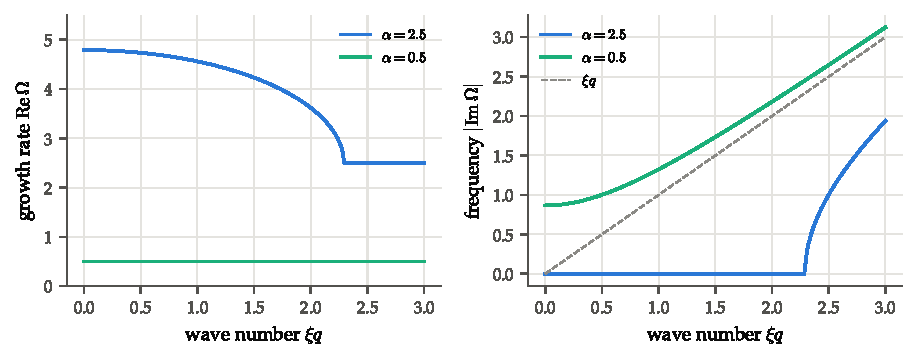
\includegraphics[width=\linewidth]{bk/dispersion.pdf}
  \caption{Linear stability of uniform sliding, \cref{eq:dispersion}. Left: growth rate of a perturbation of wave number $q$; it is
  positive for every $q$. Right: oscillation frequency; for $\xi q\gg\bar\alpha$ it approaches $\xi q$, i.e.\ short perturbations travel
  as waves with speed $\xi$.}
  \label{fig:dispersion}
\end{figure}

% ======================================================================
\section{Growing slip pulses}
\label{sec:bk-pulses}

The same instability acts during a slipping event, and Carlson and Langer use it to understand how events grow. Consider a region of
the fault in which all blocks are just at the threshold of slipping. In the continuum limit with $\nu\to0$, such a state $U_c(s)$
satisfies the force balance with friction at its maximum,
\begin{equation}
  \xi^2\,\frac{\dd^2U_c}{\dd s^2} - U_c = 1 \qquad\Longrightarrow\qquad U_c(s) = -1 + \epsilon\cosh(s/\xi)
\end{equation}
(in the frame of \cref{eq:bk-CL}), where the small constant $\epsilon$ measures how far the region is from being exactly at threshold.

Suppose a small slip starts at a point $s_0$ of this region, and write $U = U_c + \delta U$. In the slipping region friction is
$\phi\approx(1-\sigma) - 2\alpha\,\delta\dot U$ (the drop $\sigma$ plus the linear decrease with slope $-1$). Inserting this,
\begin{equation}
  \delta\ddot U = \xi^2\,\delta U'' - \delta U + \sigma + 2\alpha\,\delta\dot U .
\end{equation}
Differentiate once with respect to time to obtain an equation for the slip velocity $w = \delta\dot U$; the constant $\sigma$ drops out:
\begin{equation}
  \ddot w = \xi^2 w'' - w + 2\alpha\,\dot w .
  \label{eq:telegraph}
\end{equation}
This is a wave equation with negative damping. To solve it, separate the growth: write $w = e^{\alpha\tau}\,W$. Then
$\dot w = e^{\alpha\tau}(\alpha W + \dot W)$ and $\ddot w = e^{\alpha\tau}(\alpha^2W + 2\alpha\dot W + \ddot W)$. Substituting and
cancelling $e^{\alpha\tau}$,
\begin{equation}
  \alpha^2W + 2\alpha\dot W + \ddot W = \xi^2W'' - W + 2\alpha^2W + 2\alpha\dot W
  \quad\Longrightarrow\quad
  \ddot W = \xi^2W'' + (\alpha^2-1)\,W .
\end{equation}
For a pulse much narrower than $\xi/\sqrt{|\alpha^2-1|}$, the second derivative $W''$ is much larger than the last term, which can be
neglected. What remains is the ordinary wave equation, whose solution (d'Alembert) is two copies of the initial pulse travelling in
opposite directions with speed $\xi$. Restoring the factor $e^{\alpha\tau}$, a narrow kick at $s_0$ develops into
\begin{equation}
  \delta\dot U(s,\tau) \approx \frac{w_0}{2}\,e^{\alpha\tau}\Bigl[\delta(s-s_0-\xi\tau) + \delta(s-s_0+\xi\tau)\Bigr]:
  \label{eq:pulses}
\end{equation}
\emph{two pulses that run outward at the sound speed $\xi$ and grow exponentially at the rate $\alpha$}. Carlson \emph{et al.} take the
initial kick to be a one-block event, with $w_0 = \sigma\xi/\omega_1^2$.

\Cref{fig:pulses} shows this mechanism in the discrete chain: a numerical solution of the linearised equations of motion, started from a
short velocity kick a few blocks wide. Two pulses run outward at $\ell$ blocks per unit time and grow roughly as $e^{\alpha\tau}$. The
linear equations allow negative velocities, which the real model forbids; the linear picture is therefore valid only for the early,
small-amplitude stage of an event.

\begin{figure}[t]
  \centering
  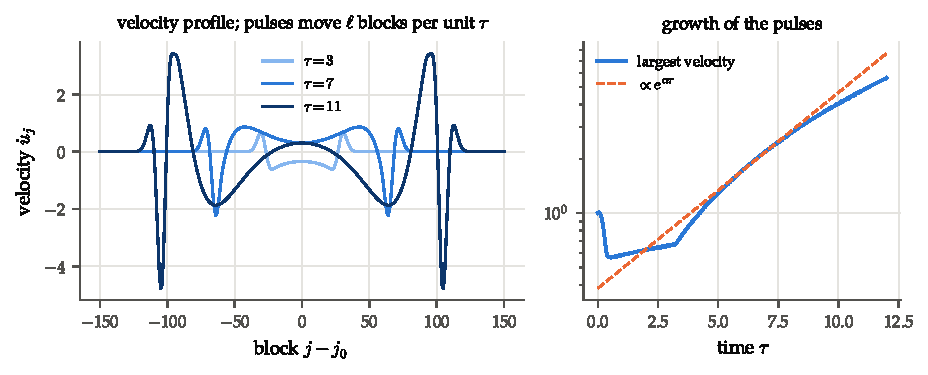
\includegraphics[width=\linewidth]{bk/pulses.pdf}
  \caption{Growing slip pulses in the linearised chain ($\ell=10$, $\alpha=0.25$, 301 blocks), started from a short velocity kick at the
  centre. Left: velocity profile at three times. Right: the largest velocity in the chain against time, compared with $e^{\alpha\tau}$.}
  \label{fig:pulses}
\end{figure}

% ======================================================================
\section{The localization length}
\label{sec:bk-localization}

The growing pulses explain why there are two kinds of large events. Suppose the region that is close to threshold, the
\emph{triggering zone}, has length $\Delta s$, and the event starts near its middle. Each pulse travels a distance $\Delta s/2$ before it
reaches the edge of the zone, which takes a time $\Delta\tau=\Delta s/(2\xi)$. Beyond the edge, the blocks are more firmly stuck. If the pulse
is still small when it gets there, it cannot push these blocks over their threshold and dies out: the event stays \emph{localized} inside
the zone. If the pulse has grown large, it breaks through and keeps going: the event becomes \emph{delocalized}.

\paragraph{The localization condition.} The displacement that a pulse produces at a point at distance $r$ from $s_0$ is the time integral
of the slip velocity there. Since $\int\delta(s_0 + r - s_0 - \xi\tau)\,\dd\tau = 1/\xi$, \cref{eq:pulses} gives
\begin{equation}
  \delta U(r) = \frac{w_0}{2\xi}\,e^{\alpha r/\xi} = \frac{\sigma}{2\omega_1^2}\,e^{\alpha r/\xi}.
\end{equation}
Carlson \emph{et al.} require that this displacement be smaller than a number of order one at the edge of the zone, $r=\Delta s/2$. With
$2\omega_1^2\approx4\ell^2$, the condition $\delta U(\Delta s/2) < 1$ reads
\begin{equation}
  \frac{\sigma}{4\ell^2}\,e^{\alpha\Delta s/(2\xi)} < 1
  \quad\Longleftrightarrow\quad
  \Delta s < \tilde\xi \equiv \frac{2\xi}{\alpha}\,\ln\frac{4\ell^2}{\sigma} .
  \label{eq:xi-tilde}
\end{equation}
Events in zones shorter than $\tilde\xi$ stay localized; longer ones run away. The \emph{localization length} $\tilde\xi$ plays the role of
a correlation length: it is the size of the largest ``ordinary'' event.

\paragraph{The crossover moment.} The total moment of a marginally localized event is the integral of the slip velocity over space and
time. Integrating \cref{eq:pulses} over $s$ gives $w_0e^{\alpha\tau}$, and integrating this over the duration $\Delta\tau = \tilde\xi/(2\xi)$,
\begin{equation}
  \tilde M = \int_0^{\Delta\tau} w_0\,e^{\alpha\tau}\,\dd\tau = \frac{w_0}{\alpha}\left(e^{\alpha\Delta\tau}-1\right)
  \approx \frac{\sigma\xi}{2\ell^2\alpha}\cdot\frac{4\ell^2}{\sigma} = \frac{2\xi}{\alpha},
  \label{eq:M-tilde}
\end{equation}
using $e^{\alpha\Delta\tau} = 4\ell^2/\sigma\gg1$ from \cref{eq:xi-tilde}. Remarkably, $\tilde M$ does not depend on $\sigma$: a smaller
$\sigma$ means a weaker initial kick, which must grow for longer, but the final moment is the same. Carlson \emph{et al.} stress that these
estimates set only the \emph{scales}; the numerical prefactors are not reliable.

\paragraph{The 1989 version.} In the 1989 paper the kick is set by the loading speed $\nu$ instead of $\sigma$, and the localization criterion is
that the displacement at the edge be smaller than $\ell^{-2}$ (the displacement needed to push a neighbour over threshold through one coupling
spring), giving~\cite{CarlsonLanger1989}
\begin{equation}
  \tilde\xi_{1989} \approx \frac{2\xi}{\alpha}\,\ln\frac{4\xi}{\nu a},\qquad \tilde M \approx\frac{2\xi}{\alpha}.
\end{equation}
For their main parameters ($\ell=10$, $\alpha=2.5$, $\nu=0.01$) this gives $\tilde\xi\approx66\,a$, compared with system sizes $N=100$--$400$.

\paragraph{The critical parameter.} In both versions $\tilde\xi$ grows logarithmically without bound as the triggering parameter goes to zero
($\sigma\to0$ in 1991, $\nu\to0$ in 1989). This parameter therefore plays the role of the distance from a critical point: only in the limit
$\sigma\to0$ does the range of localized events become infinite. The logarithmic dependence means, however, that this limit is approached very
slowly (\cref{fig:localization}). For the parameters of the 1991 paper ($\alpha=3$, $\sigma=0.01$) the localization length is about 38 blocks for
$\ell=6$ and 88 blocks for $\ell=12$, while the smallest and crossover moments are $M_1\approx2.7\times10^{-4}a$ and $\tilde M=4a$ for $\ell=6$: the
localized events span about four decades in moment.

\begin{figure}[t]
  \centering
  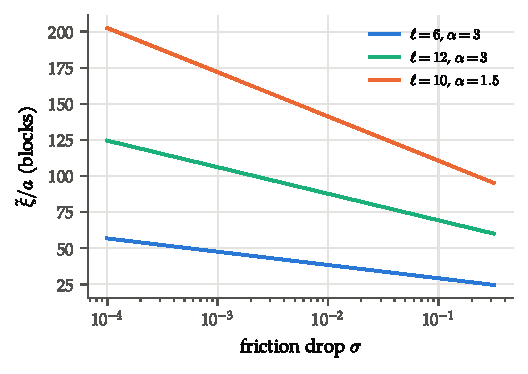
\includegraphics[width=0.55\linewidth]{bk/localization.pdf}
  \caption{Localization length \cref{eq:xi-tilde}, in units of the block spacing, as a function of the friction drop $\sigma$.}
  \label{fig:localization}
\end{figure}

% ======================================================================
\section{Three kinds of events and the cycle of the fault}
\label{sec:bk-events}

Carlson and Langer found that the events of the model fall into three classes, each with its own physics:
\begin{enumerate}
  \item \textbf{Microscopic events}, involving one or a few blocks (\cref{sec:one-block-event}). Their moments are of order $M_1 = 2\sigma a/(2\ell^2+1)$
    and come in discrete steps (\cref{eq:Mn}). They release very little stress and mainly smooth the configuration on the scale of a few blocks.
  \item \textbf{Localized events}, larger than microscopic but smaller than the localization length, with moments up to about $\tilde M = 2\xi/\alpha$.
    These form the broad, power-law ``scaling region'' of the size distribution.
  \item \textbf{Delocalized events}, in which the pulses break out of the triggering zone. They propagate along the fault at the sound speed, can
    involve hundreds or thousands of blocks, and displace them by amounts of order one. They are much more frequent than an extrapolation of the
    scaling region would predict.
\end{enumerate}

The 1991 paper describes how the classes are related (its Fig.~2, which shows a sequence of stuck configurations). After a large delocalized event the
configuration is rough on all scales below $\tilde\xi$, because the instability of \cref{sec:bk-instability} amplifies irregularities while the blocks slip.
The many small and localized events that follow do not move the fault much; their main effect is to \emph{smooth} the configuration: a group of blocks that
lags behind its neighbours slips and catches up. Once a region of size about $\tilde\xi$ has become smooth enough and reaches the threshold, it triggers the
next delocalized event, which roughens the configuration again. In this picture the localized events are not an independent self-organized critical
process: their statistics are controlled by the delocalized events, which set up the rough configurations that the small events then smooth out.

% ======================================================================
\section{Statistics of events}
\label{sec:bk-stats}

\subsection{Definitions}

The \emph{moment} of an event is the total slip it produces, in units of $D_0$ times the block spacing:
\begin{equation}
  M = a\sum_{j}\delta U_j ,
\end{equation}
where $\delta U_j$ is the displacement of block $j$ during the event and the sum runs over the blocks that moved. Its magnitude is $\mu = \ln M$
(Chapter~\ref{ch:intro}). Carlson and Langer use $a=1$, so $M$ is the sum of the block displacements.

In the 1989 paper, with a finite loading speed, the distribution of events is described by $\mathcal R(\mu)$, the number of events \emph{per unit time
and per unit length} of the fault with magnitude between $\mu$ and $\mu+\dd\mu$. In the limit $\nu\to0$ of the 1991 paper, time has no meaning between events,
and the natural quantity is the number of events \emph{per unit plate displacement} and per unit length,
\begin{equation}
  \mathcal D(\mu) = \frac{\mathcal R(\mu)}{\nu}.
\end{equation}

\paragraph{The sum rule.} Over a long time $T$ the plate moves by $\nu T$, and every block must on average move by the same amount (otherwise its pulling
spring would stretch without limit). The total moment of all events in time $T$ on a fault of length $L$ is therefore $L\,\nu T$. Since the number of events
in $\dd\mu$ is $\mathcal R(\mu)\,\dd\mu\, L T$, each with moment $e^\mu = M$,
\begin{equation}
  \int M\,\mathcal R(\mu)\,\dd\mu = \nu,\qquad\text{equivalently}\qquad \int M\,\mathcal D(\mu)\,\dd\mu = 1 .
  \label{eq:sumrule}
\end{equation}
This exact constraint links the frequencies of small and large events: if the small events do not move the fault forward enough, large events must do it.

\subsection{The 1989 results}

Carlson and Langer simulated chains of $N=100$ to $400$ blocks with $\ell=10$, $\nu=0.01$ and $0.001$, and $\alpha$ from 1 to 4, over $40$ to $1000$ loading
periods $2/\nu$. Their distributions $\ln\mathcal R(\mu)$ show:
\begin{itemize}[nosep]
  \item at small $\mu$, sharp peaks from the one-block and few-block microscopic events;
  \item in the middle, a straight ``scaling region'' $\mathcal R\propto e^{-b\mu}$ with $b\approx1$ for $\alpha\gtrsim2.5$; for smaller $\alpha$ the slope is
    flatter ($b\approx0.35$ at $\alpha=1$);
  \item at large $\mu$, a bump of delocalized ``great'' events, near the largest possible moment $\mu_L=\ln(2N)$ (all blocks displaced by 2).
\end{itemize}
They explained the scaling region with a dimensional argument. In the continuum equation \cref{eq:bk-cont} the only length is $\xi$, so if neither $a$ nor
$N$ matters in the scaling region, $\mathcal R$ can depend on $M$ only through $M/\tilde M = \alpha M/2\xi$:
\begin{equation}
  \mathcal R_S(\mu) = \frac{\nu}{M}\,\mathcal C\!\left(\frac{\alpha M}{2\xi},\alpha\right)
  \;\approx\; \frac{\nu}{M}\,\mathcal C_0(\alpha)\left(\frac{\alpha M}{2\xi}\right)^{\eta}\qquad (M\ll\tilde M).
\end{equation}
Comparing with $\mathcal R\propto e^{-b\mu} = M^{-b}$ gives $b = 1-\eta$; $b=1$ corresponds to $\eta=0$, a power law with no ``anomalous dimension''. In the language
of Chapter~\ref{ch:intro}, $b = 1$ means a moment density $P(M)\propto M^{-2}$, $\tau=2$.

The authors note several limitations of their data. The great events appear roughly once per loading period, and the runs covered between 40 and 1000 loading
periods, so the large-event part of the distribution rests on relatively few events. The system sizes were only a few times the localization length
($\tilde\xi\approx66$ for $N=100$), and they observed that the distributions depend on $N$ near the upper end. Finally, the finite loading speed introduces
another length, $2\xi/\nu$, the distance a sound wave travels in one loading period; for $\nu=0.01$ and large $N$ they found resonant propagating modes in which
the picture of separate events breaks down.

\subsection{The 1991 results}

With the $\sigma$ friction law and $\nu\to0$, Carlson, Langer, Shaw and Tang simulated much longer chains: $N=4096$ and $8192$, with $\alpha=3$, $\sigma=0.01$ and
$\ell=6$, 8 and 12 (their Fig.~3), so that even the largest events never span the whole system. Their main findings are:
\begin{itemize}
  \item The distribution $\mathcal D(\mu)$ has a scaling region of localized events with slope $b\approx0.92$ (from a least-squares fit), a pronounced minimum
    just below $M=\tilde M$, and a peak of delocalized events. The minima for different $\ell$ coincide when plotted against $\ln(M/\xi)$, confirming that the
    crossover is at $M\approx\tilde M\propto\xi$.
  \item They summarise the distribution as
    \begin{equation}
      \mathcal D(\mu)\approx
      \begin{cases}
        A\,(\tilde M/M)^{b}, & M_1<M<\tilde M,\\
        A'\,(M/M^*)^{-b'}, & \tilde M<M<M^*,\\
        0, & M<M_1\ \text{or}\ M>M^*,
      \end{cases}
      \label{eq:D91}
    \end{equation}
    with $b\approx1$ and $b'\approx-1$: the delocalized events \emph{rise} with $M$ up to a sharp upper cutoff $M^*$.
  \item The upper cutoff grows with $\ell$ faster than $\tilde M$, roughly as $M^*/\tilde M\propto\ell$ for large $\alpha$. Because the ratio depends on
    $\ell=\xi/a$ and not only on $\xi$, the block spacing $a$ (the ``ultraviolet cutoff'') matters: the model has no simple continuum limit.
  \item For small $\alpha$ ($\alpha=1$, $\sigma=0.01$, $\ell=6$, 10, 14) the separation between localized and delocalized events disappears, and the whole
    distribution is a single power law with $b\approx0.35$.
  \item The localization length measured from the distribution of the number of blocks per event is of the order of $\tilde\xi$ but typically larger than
    \cref{eq:xi-tilde}.
\end{itemize}
Translated into the moment density $P(M)$ (\cref{eq:CL-b-tau}), $b\approx1$ in the localized region means $\tau\approx2$, $b'\approx-1$ for the delocalized events
means $P(M)\approx$ constant up to $M^*$, and $b\approx0.35$ at $\alpha=1$ means $\tau\approx1.35$.

% ======================================================================
\section{Why the two papers differ}
\label{sec:bk-differences}

\Cref{tab:89vs91} collects the differences between the two studies. They are not two runs of the same model with more or less data: they are different models,
analysed in different limits, with different observables. A simulation that mixes features of both, for example the friction drop of 1991 with a finite loading
speed and the event definition of 1989, cannot be expected to reproduce either. Even within one model, the 1989 runs were short and the systems small compared
with the length scales involved, which makes the delocalized part of the distribution and the shape near the crossover statistically fragile.

\begin{table}[t]
\centering
\caption{The two studies of the BK model by Carlson and collaborators.}
\label{tab:89vs91}
\begin{tabular}{@{}lp{55mm}p{55mm}@{}}
\toprule
 & 1989~\cite{CarlsonLanger1989} & 1991~\cite{Carlson1991} \\
\midrule
friction at rest & $[-1,1]$; backward slip possible & $(-\infty,1]$; no backward slip \\
onset of slip & smooth, friction starts at 1 & abrupt drop to $1-\sigma$ \\
loading speed & finite, $\nu = 0.01$, $0.001$ & $\nu\to0$ (event-driven) \\
critical parameter & $\nu$ & $\sigma$ \\
localization length & $\frac{2\xi}{\alpha}\ln\frac{4\xi}{\nu a}$ & $\frac{2\xi}{\alpha}\ln\frac{4\ell^2}{\sigma}$ \\
distribution & $\mathcal R(\mu)$ per unit time & $\mathcal D(\mu)=\mathcal R/\nu$ per unit displacement \\
system size & $N = 100$--$400$ & $N = 4096$--$8192$ \\
stiffness & $\ell = 10$ & $\ell = 6$, 8, 12 (and 3, 10, 14) \\
duration of runs & 40--1000 loading periods & hundreds to thousands of loading periods \\
\bottomrule
\end{tabular}
\end{table}

For this thesis we therefore take the 1991 model as the reference: its definition is cleaner (no dependence on $\nu$), its simulations are larger, and it is the one
that maps most naturally onto a sandpile, where grains are also added only when all activity has stopped. The 1989 model with finite $\nu$ is treated afterwards, as a
variation.

% ======================================================================
\section{Summary: what a sandpile would have to capture}
\label{sec:bk-summary}

The analysis of this chapter identifies the ingredients that determine the statistics of the BK model:
\begin{enumerate}
  \item \textbf{A threshold with a drop.} A block slips when its spring force reaches the static threshold, and then sheds a force $\Delta f$ of order $\sigma$ (\cref{sec:one-block-event}).
    This is the analogue of a sandpile site toppling when its height reaches the critical value.
  \item \textbf{Redistribution with bulk dissipation.} Of the force shed, a fraction $2\ell^2/(2\ell^2+1)$ goes to the two neighbours and a fraction
    $\epsilon = 1/(2\ell^2+1)$ is lost into the pulling spring. In sandpile language this is a toppling rule with bulk dissipation $\epsilon$, which introduces a length
    of order $\ell$, the stiffness length.
  \item \textbf{Uniform, deterministic driving.} The plate loads all blocks at the same rate, and in the limit $\nu\to0$ it is moved only between events, exactly like a
    sandpile that is driven only when it is stable.
  \item \textbf{Inertia and velocity weakening.} Slipping blocks have velocities, and velocity-weakening friction amplifies slip pulses at the rate $\alpha$
    (\cref{sec:bk-pulses}). This is what produces the delocalized events and the localization length $\tilde\xi\propto(\xi/\alpha)\ln(4\ell^2/\sigma)$. A sandpile, whose
    topplings have no memory of velocity, has no counterpart of this ingredient.
\end{enumerate}
The first three ingredients define a sandpile model of the Olami--Feder--Christensen type. Chapter~5 derives this model from \cref{eq:bk} and asks how much of the BK
statistics survives when the fourth ingredient, inertia, is removed. The answer to that question is the central result of this thesis.
